% Generated by scripts/build_unified_paper.py from paper/unified-contextuality.md.  Compile with XeLaTeX or LuaLaTeX.
\documentclass[11pt,a4paper]{article}
\usepackage{fontspec}
\setmonofont{DejaVuSansMono.ttf}[Scale=0.82]
\usepackage[margin=1in]{geometry}
\usepackage{amsmath,amssymb}
\usepackage{graphicx}
\usepackage{longtable,booktabs,array,calc}
\usepackage{fvextra}
\usepackage{xurl}
\usepackage[colorlinks=true,linkcolor=black,citecolor=black,urlcolor=blue]{hyperref}
\RecustomVerbatimEnvironment{verbatim}{Verbatim}{breaklines=true,breakanywhere=true,fontsize=\footnotesize}
\providecommand{\tightlist}{\setlength{\itemsep}{0pt}\setlength{\parskip}{0pt}}
\providecommand{\pandocbounded}[1]{#1}
\newcommand{\lt}{<}
\newcommand{\gt}{>}
\setlength{\emergencystretch}{3em}
\setlength{\parskip}{0.45em}
\setlength{\parindent}{0pt}
\setcounter{secnumdepth}{0}
\renewcommand{\arraystretch}{1.15}
\makeatletter
\def\maxwidth{\ifdim\Gin@nat@width>\linewidth\linewidth\else\Gin@nat@width\fi}
\makeatother
\setkeys{Gin}{width=\maxwidth,keepaspectratio}

\hypersetup{pdftitle={Spectral bounds and their limits in Pauli contextuality: exact configurations and a proof of Jonah\textquotesingle s Conjecture E},pdfauthor={Alexander S. Donahue; 0thernes LLC}}


\title{Supplementary material\\[0.5em]\large Spectral bounds and their limits in Pauli contextuality: exact configurations and a proof of Jonah\textquotesingle s Conjecture E}

\author{Alexander S. Donahue\\0thernes LLC, Washington, USA\\ORCID \href{https://orcid.org/0009-0006-8168-9648}{0009-0006-8168-9648}\\\texttt{0\_0@0thernes.art}}

\date{}

\begin{document}

\maketitle

Hoggar Bound Lab, version 1.3.0, 10 November 2026. Research preprint. Not peer reviewed.
Research and manuscript preparation used Claude (Anthropic) and OpenAI Codex agents under the author\textquotesingle s direction; see Section 13.

This journal-format document is derived from the complete paper, version 1.3.0. Original section numbers and cross-references are retained; gaps are intentional. The supplement contains: 10. A running example on the Tsotchke stack, 11. Falsifiability and replication, Appendix A. Reproduction, Appendix B. Witness assignments. References are reproduced in both journal documents.

\subsection{10. A running example on the Tsotchke stack}\label{10-a-running-example-on-the-tsotchke-stack}

\subsubsection{10.1 State preparation, simulated contexts and quantum geometry}\label{101-state-preparation-simulated-contexts-and-quantum-geometry}

All four components are used for what they are.

\begin{itemize}
\tightlist
\item
  \textbf{Moonlab} (v1.2.1, prebuilt WebAssembly engine) is a classical state-vector simulator. It plays
  the quantum device.
\item
  \textbf{quantum\_rng} is a classical, "quantum-inspired" integer and trigonometric mixer, not a hardware
  quantum source. It supplies seeded pseudo-random numbers. Its stream depends on the C library it is
  built against, so no result depends on its exact values: every count is recomputed independently.
\item
  \textbf{QGTL} (quantum\_geometric\_tensor): only the \texttt{diffgeo\_*} kernels (Fubini--Study metric, Berry
  curvature), which we had verified earlier against closed forms, are used.
\item
  \textbf{Eshkol} (v1.3.6) is a Scheme dialect with automatic differentiation. It carries an independent
  implementation of the geometry and the differentiation checks.
\end{itemize}

\textbf{Experiment on Moonlab, classical families} (\nolinkurl{src/moonlab_experiment.mjs}, seed 20261109). A Pauli
observable is measured projectively by rotating its eigenbasis onto \(Z\) of one qubit (gates \(H\),
\(S^\dagger\), CNOT), calling Moonlab\textquotesingle s single-qubit measurement with a number from quantum\_rng, and
undoing the rotation.

{\def\LTcaptype{none} % do not increment counter
{\small
\begin{longtable}[]{@{}>{\raggedright\arraybackslash}p{(\linewidth - 4\tabcolsep) * \real{0.0505}}>{\raggedright\arraybackslash}p{(\linewidth - 4\tabcolsep) * \real{0.4748}}>{\raggedright\arraybackslash}p{(\linewidth - 4\tabcolsep) * \real{0.4748}}@{}}
\toprule\noalign{}
step & what is done & result \\
\midrule\noalign{}
\endhead
\bottomrule\noalign{}
\endlastfoot
E0 & Moonlab\textquotesingle s \(\langle P\rangle\) against a direct evaluation; repeated measurement & agree to \(8.6\times10^{-16}\); repeats agree \\
E1 & \(\psi_H\) on 3 simulated qubits; 63 expectation values; signs as an assignment & all \(\pm 1/3\) (to \(6\times10^{-16}\)); 63 of 315 contexts violated, three through each point \\
E2 & realified \(\psi_H\) on 4 simulated qubits & \(\pm 1/3\) on 135 real observables, \(0\) on 120 imaginary ones; 315 of 1575 violated, seven through each point \\
E3 & every context measured sequentially on random states, \(N = 2,3,4\), three runs each & \(15/15\), \(315/315\), \(5355/5355\) products equal to the quantum sign (16065 projective measurements and 161406 gates per four-qubit run) \\
E4 & the same with a random Pauli error of probability \(p\) on each qubit before each measurement; 3000 to 4000 sampled contexts & Figure 4 and the table below \\
\end{longtable}
}
}

The table reports the fraction of sampled contexts whose outcomes multiply to the quantum sign,
against proved noncontextual ceilings. For three and four qubits the ceiling is
\(1-d_{\text{floor}}/L\). The two-qubit column uses the independently known exact degree \(d=3\),
giving \(1-3/15=0.800\); the spectral floor alone rounds to 2 there.

{\def\LTcaptype{none} % do not increment counter
{\small
\begin{longtable}[]{@{}>{\raggedright\arraybackslash}p{(\linewidth - 6\tabcolsep) * \real{0.5221}}>{\raggedright\arraybackslash}p{(\linewidth - 6\tabcolsep) * \real{0.1593}}>{\raggedright\arraybackslash}p{(\linewidth - 6\tabcolsep) * \real{0.1593}}>{\raggedright\arraybackslash}p{(\linewidth - 6\tabcolsep) * \real{0.1593}}@{}}
\toprule\noalign{}
error \(p\) & \(N=2\) & \(N=3\) & \(N=4\) \\
\midrule\noalign{}
\endhead
\bottomrule\noalign{}
\endlastfoot
0 & 1.000 & 1.000 & 1.000 \\
0.01 & 0.979 & 0.969 & 0.957 \\
0.02 & 0.958 & 0.939 & 0.930 \\
0.05 & 0.897 & 0.867 & 0.830 \\
0.10 & 0.805 & 0.747 & 0.717 \\
0.20 & 0.669 & 0.616 & 0.591 \\
ceiling, proved & 0.800 & 0.800 & 0.729 \\
best classical model known & 0.800 & 0.800 & 0.706 \\
\end{longtable}
}
}

\textbf{Experiment on Moonlab, the configurations of Table 1} (\nolinkurl{src/moonlab_saturated.mjs}, seed 20261110).

{\def\LTcaptype{none} % do not increment counter
{\small
\begin{longtable}[]{@{}>{\raggedright\arraybackslash}p{(\linewidth - 4\tabcolsep) * \real{0.0505}}>{\raggedright\arraybackslash}p{(\linewidth - 4\tabcolsep) * \real{0.4748}}>{\raggedright\arraybackslash}p{(\linewidth - 4\tabcolsep) * \real{0.4748}}@{}}
\toprule\noalign{}
step & what is done & result \\
\midrule\noalign{}
\endhead
\bottomrule\noalign{}
\endlastfoot
S1 & the first six states of Table 1 loaded as amplitudes; \(\Phi_5\) and \(\Phi_7\) prepared by running their circuits (Hadamard, controlled-phase and Toffoli gates of Moonlab: 14 and 34 gates); every Pauli expectation value read through Moonlab\textquotesingle s gates & the circuits give the phase states to \(10^{-16}\); non-zero expectation values of one modulus to \(10^{-15}\); supports and signs equal the masks in \texttt{data/flat/}; contexts and violated contexts as in Table 1, including 2 824 192 and 729 344 for seven qubits \\
S2 & every context of \(S_B\) (three runs), of \(S_5\) and of the support of \(\Phi_5\) measured sequentially on random states; for \(S_7\) a sample of 30000 contexts, and once all of them & \(1095/1095\), \(10880/10880\), \(10880/10880\), \(30000/30000\) products equal to the quantum sign; in the full seven-qubit run \(2\,824\,192/2\,824\,192\) (8 472 576 projective measurements, 161 550 336 gates) \\
S3 & the same with Pauli noise; 4000 sampled contexts & the table below \\
\end{longtable}
}
}

Because the degrees are exact, the ceilings in this table are exact as well: \(1 - d/L\). For the four-
and five-qubit configurations they are much higher than for the full space, so the test tolerates much
less noise; for \(S_7\) the ceiling is \(0.742\) and the simulated test stays above it up to an error
probability of two per cent per qubit and measurement.

{\def\LTcaptype{none} % do not increment counter
{\small
\begin{longtable}[]{@{}>{\raggedright\arraybackslash}p{(\linewidth - 8\tabcolsep) * \real{0.1756}}>{\raggedright\arraybackslash}p{(\linewidth - 8\tabcolsep) * \real{0.2105}}>{\raggedright\arraybackslash}p{(\linewidth - 8\tabcolsep) * \real{0.2105}}>{\raggedright\arraybackslash}p{(\linewidth - 8\tabcolsep) * \real{0.1846}}>{\raggedright\arraybackslash}p{(\linewidth - 8\tabcolsep) * \real{0.2188}}@{}}
\toprule\noalign{}
error \(p\) & \(S_B\) (four qubits) & \(S_5\) (five qubits) & support of \(\Phi_5\) & \(S_7\) (seven qubits) \\
\midrule\noalign{}
\endhead
\bottomrule\noalign{}
\endlastfoot
0 & 1.000 & 1.000 & 1.000 & 1.000 \\
0.002 & 0.992 & 0.989 & 0.990 & 0.986 \\
0.005 & 0.982 & 0.981 & 0.978 & 0.963 \\
0.01 & 0.962 & 0.955 & 0.949 & 0.938 \\
0.02 & 0.929 & 0.913 & 0.916 & 0.877 \\
0.05 & 0.835 & 0.807 & 0.797 & 0.733 \\
0.10 & 0.719 & 0.679 & 0.670 & 0.597 \\
ceiling, exact & 0.932 & 0.956 & 0.956 & 0.742 \\
\end{longtable}
}
}

These are frequencies in a seeded software simulation. They illustrate the inequalities and are not
measurements on hardware or a loophole analysis.

\pandocbounded{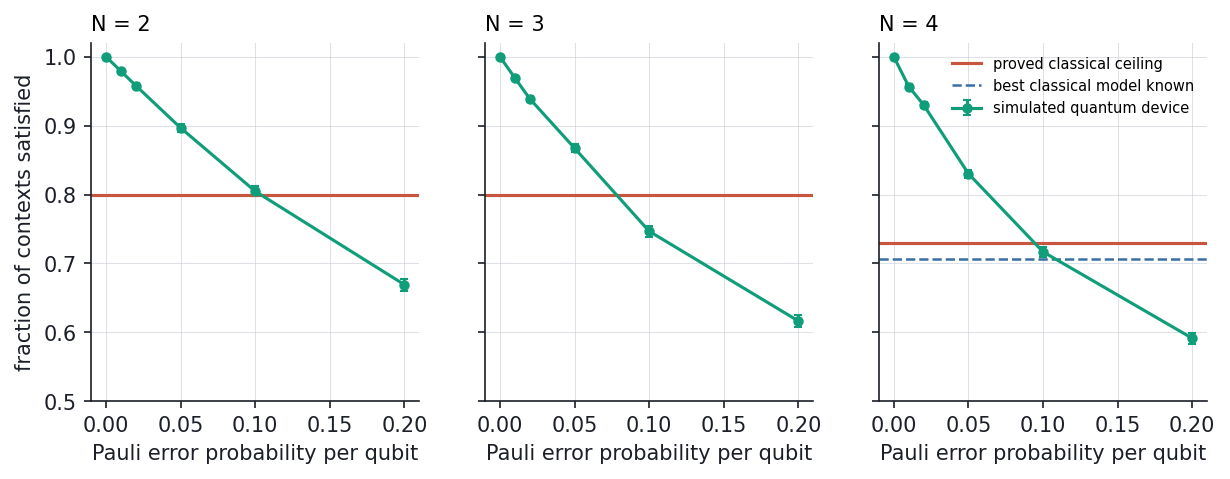
\includegraphics[keepaspectratio,alt={Figure 4}]{figures/fig2_noise.png}}

\emph{Figure 4. Simulated success fraction on Moonlab against the classical ceilings, for the full space.}

\textbf{QGTL} (\texttt{src/qgt\_hoggar.c}, \texttt{src/qgt\_flat.c}). The kernels \nolinkurl{diffgeo_compute_fubini_study} and
\nolinkurl{diffgeo_compute_berry_curvature}, applied to \(\psi_H\) and the 63 tangent vectors \(-\tfrac{i}{2}P_v\psi_H\),
return the values of Proposition 3 to \(10^{-16}\), and the 189 pairs with \(|g_{uv}| \gt 1/12\) are exactly
the pairs on the 63 violated contexts. For the eight states of Table 1 and the tangent vectors of their
supports they return the three values of Proposition 8 to \(10^{-16}\); the pairs above the threshold
recover the 75 violated contexts of \(S_B\) (225 pairs of 9045), the 480 of \(S_5\) and of the support of
\(\Phi_5\) (1440 pairs of 122760), and the 729 344 of \(S_7\) (2 188 032 pairs of 33 028 128), and no others.

\textbf{Eshkol} (\texttt{src/eshkol/hoggar.esk}, \nolinkurl{src/eshkol/saturated.esk}). An exhaustive pass over all \(2^{15}\)
two-qubit assignments gives minimum 3, attained 640 times. The Hoggar signs violate 63 contexts.
Reverse-mode automatic differentiation of the cubic form at the Hoggar Pauli vector \(x^\ast\) gives
\(T(x^\ast) = 7 = (D-1)(D-2)/6\) and \(\nabla T(x^\ast) = 3x^\ast\) to \(7\times10^{-16}\) (the Lagrange condition
for a maximizer on the sphere); nested forward-mode second derivatives along four tangent directions are
negative (\(-0.59\) to \(-0.74\)). For the pivot state the second script finds 135 non-zero expectation
values, 1095 contexts and 75 violated ones, \(T = 35 = (D-1)(D-2)/6\), and \(\nabla T = 7x\) to
\(1.3\times10^{-15}\), which is condition (d) of Theorem 4.

\subsubsection{10.2 Exact C3 arithmetic in Eshkol}\label{102-exact-c3-arithmetic-in-eshkol}

The separate serial compiled run uses Eshkol 1.3.6-evolve through
\texttt{eshkol-run\ -r}. It checks \(A_0M=MA_1\) and both \(MR=RM=46656I\), then evaluates the block-moment
formula to obtain 14976 and 15360. An arbitrary-precision Python replay bounds every input, product
and ordered accumulation of this program by 408304 in absolute value, below \(2^{63}-1\). The recorded
run returned zero with empty standard error; \nolinkurl{results/frontier-c3-eshkol.json} records its command,
hashes and process-local paths to the existing LLVM 21 and CUDA 12.9 installations. This qualifies
the tested serial arithmetic execution, not compiler correctness or GPU/parallel behavior.

\subsection{11. Falsifiability and replication}\label{11-falsifiability-and-replication}

\subsubsection{11.1 Floor, saturation and simulated measurement checks}\label{111-floor-saturation-and-simulated-measurement-checks}

\textbf{Predictions that could fail.} (P1) No assignment violates fewer contexts than the floor. (P2) The
saturated cases are reached exactly. (P3) For every \(S\) and \(f\), \(\operatorname{tr}A = 0\),
\(\operatorname{tr}A^2 = D|S|\), \(\operatorname{tr}A^3 = 6D\beta\). (P4) On an elliptic quadric the spectrum of
\(A\) is doubly degenerate. (P5) For every pure state \(T(p) = (D-1)(D-2)/6\). (P6) Ideal sequential
measurements reproduce every context sign in every state. (P7) For a flat state, condition (d) of
Theorem 4 holds. A counterexample to P1 would provide a finite assignment whose violation count can
be recomputed independently from the context definitions.

\textbf{Tests} (\texttt{scripts/run\_all.sh}).

\begin{itemize}
\tightlist
\item
  \texttt{hoggar\ exhaust2}: all 32768 two-qubit assignments; minimum 3 (640 assignments); for the square,
  minimum 1.
\item
  \texttt{scripts/run\_falsify.sh}: 20 runs over \(N = 2, \dots, 5\) and the three families; 20000, 5000 and 500
  uniformly random assignments and 1500, 200 and 12 annealed ones per configuration for
  \(N = 3, 4, 5\). No assignment below the floor. Minima reached by annealing: 63, 21, 9 (\(N=3\));
  1575, 315, 315 (\(N=4\)); 31479, 6975, 7087 (\(N=5\)). These equal the best known values in every case.
\item
  A negative control: the false claim \(d(W(5,2)) \ge 64\) is refuted by the Hoggar witness with exit
  code 3, showing that the harness can fail.
\item
  \texttt{scripts/flat\_states.py} (68 checks, integer arithmetic in \(\mathbb{Z}[i]\) except one labelled check):
  for the six states of Table 1, the single modulus, the support, the number of contexts, the number
  violated, the floor, condition (d) at every point and the vanishing of every outside sum; the statements
  of Theorem 5 about \(S_B\); Proposition 6 on all 4096 phase patterns; Proposition 9 for one to four
  qubits; and an annealing search from random starts on \(S_B\) and \(S_5\), which reaches 75 and 480 and
  never goes below.
\item
  \texttt{build/third\_level} (seven seconds): the enumeration of Theorem 12, all 33 554 431 forms for five
  qubits included, with the orbit computation; it fails if any count differs from the table.
\item
  \texttt{scripts/phase\_states.py} (81 checks, integer arithmetic): for \(CS|{+}{+}\rangle\), \(CCZ|{+}{+}{+}\rangle\),
  \(CS\,CS|{+}{+}{+}\rangle\), \(\Phi_5\) and \(\Phi_7\), the constant rank, the single modulus, the support, the
  numbers of contexts and violated contexts, condition (d) and the outside sums, and the description of
  the support in Proposition 11; Proposition 10 for all eleven states of this paper; the enumeration of
  Theorem 12 for \(N \le 4\) by a second implementation; the two symplectic maps of Theorem 12; and the
  finite-field descriptions of the five- and seven-qubit forms.
\item
  \texttt{scripts/run\_family7.sh} (about eight core-hours, not part of the everyday run): the enumeration of
  Theorem 13, the orbit computation, and the random census of the other types; its output is
  \texttt{results/family7.log}. The two counts agree: 13 271 040 solutions found, and
  \(92\,897\,280/7 = 13\,271\,040\) for one orbit with a stabilizer of order 7.
\item
  The seven-qubit numbers 8128, 2 824 192 and 729 344 are computed three times without shared code: in
  Python with exact integers, in C from the masks (inside the QGTL program) and in JavaScript from the
  expectation values returned by Moonlab; and a fourth time by \nolinkurl{scripts/phase_seven_lean.py} (14
  checks), with the evaluation that the kernel carries out, compared with the direct double loop and
  with two negative controls.
\item
  \texttt{scripts/analysis.py} (62 checks) and \texttt{scripts/ladder.py} (14 checks): P3 on random data to machine
  precision; P4 on all 120 four-qubit elliptic quadrics; P5; the geometry of the violated sets; closed-form
  counts against enumeration; agreement of the C and Python integer bounds.
\item
  Witness files (\texttt{data/witness/}, \texttt{data/flat/}) are recounted by independent routines that use no tables.
\end{itemize}

\textbf{Independent implementations.} The geometry, the context signs and the counts are implemented five
times: C (\texttt{src/hoggar.c}), Python with explicit matrices or exact integers (\texttt{scripts/analysis.py},
\texttt{scripts/flat\_states.py}), JavaScript (\nolinkurl{src/moonlab_experiment.mjs}, \nolinkurl{src/moonlab_saturated.mjs}),
Eshkol, and the Lean model, in which the signs are theorems about matrix products. Their overlapping
checks agree on the counts recorded for those tests. This does not mean that each implementation
checks every result: in particular, the C3 checks use the separate programs described next.

\subsubsection{11.2 Independent C3 reconstruction and negative controls}\label{112-independent-c3-reconstruction-and-negative-controls}

The literal-matrix verifier builds each four-qubit Pauli from the \(2\times2\) matrices, selects the
real quadric and section, and computes exact carrier characteristic polynomials. A change-of-basis
matrix \(T\) with \(T^{\mathsf T}T=TT^{\mathsf T}=8I\) intertwines the completion matrix and the block
Jordan representation, checking that the coordinate transformation loses no component.

A separate verifier constructs the completion matrix from all 1120 outside signed contexts. It
checks commutation and multiplies each triple to determine its sign, then recomputes both carrier
polynomials and completion cube traces. This route does not use (C7). Its last three tensor factors
are reversed relative to the printed convention; that fixed orthogonal basis permutation is recorded
explicitly and preserves the represented assignments and spectra. Pauli entries \(0,\pm1,\pm i\) are
exact in their initial representation, real matrices are converted to integers, and product bounds
fit signed 64-bit arithmetic. Characteristic polynomials use exact SymPy arithmetic, not eigenvalue
tolerances.

Flipping one off-diagonal context entry and its symmetric partner changes the two cubic traces to
14808 and 15144 respectively, so the expected certificate fails. The verifier rejects Python \texttt{-O},
which would disable its assertions. These are specified negative controls, not a proof that every
possible implementation error is detected.

The interactive C3 model independently constructs context signs, computes characteristic polynomials
with a BigInt Faddeev--LeVerrier recurrence and evaluates cube traces with BigInt arithmetic. Editing a
sign triggers a fresh computation. A modified assignment is not required to retain cospectrality;
the original four-negative-word witnesses are the exact claim being tested. The experiments concern
finite mathematical operators and are separate from the Moonlab measurement simulations.

A further reconstruction, \nolinkurl{scripts/cospectral_pair.py} (30 checks), shares no code with these
programs. It rebuilds the 135 points, the 1575 contexts and their signs by two routes, the carrier and
block polynomials, the identity between each completion matrix and \(M\mapsto\frac12(CM+MD)\), both degree-64
completion polynomials, the enclosure of \(\rho\) and the two witnesses of Corollary 16.

\subsubsection{11.3 Checks of the carrier families}\label{113-checks-of-the-carrier-families}

\begin{itemize}
\tightlist
\item
  \texttt{scripts/cospectral\_family.py\ -\/-six} (43 checks): for \(N=3,4,5,6\) it builds every real Pauli matrix,
  the section, all outside contexts and their signs (from a phase formula and, up to five qubits, from
  products of three matrices), both carriers of Theorem 17 and both completion matrices, and checks in
  integers the block and graph forms (E5), equal characteristic polynomials, the identity of step (v)
  on all \(k^2\) blocks, (E6) against the direct cubic trace, the difference (E3) and the points where the
  carriers differ. It repeats this for 12 random graphs with random sets of components at three and
  four qubits, and has two negative controls: moving an edge that is not a whole component, or the
  component that contains \(t\), must destroy cospectrality.
\item
  \nolinkurl{scripts/cospectral_family_tensor_check.py} (18 checks) takes only the two sign tables from the first
  program, builds every observable as a Kronecker product of literal \(2\times2\) matrices, decides
  reality, commutation and context signs from matrix products, and compares power sums
  \(\operatorname{tr}A^k\) for all \(k\le2^N\) and the completion traces.
\item
  \nolinkurl{scripts/cospectral_family_cone_lift.py} (21 checks) builds the C11 configurations with 4, 5 and 6
  qubits from the definitions, without the lifting lemma, and checks the lifted pairs of Table 5.
\item
  \texttt{scripts/conjecture\_e.py} (81 checks; with the argument \texttt{6} a further 36 checks at six qubits, record
  \nolinkurl{results/conjecture_e_n6.json}) builds every vertex case at four and five qubits, and at three
  qubits for C1, C3, C6 and C11, from the definitions of {[}J3{]}: the type of the quadric and of \(e\) and \(d\)
  as in {[}J3, Table 1{]}, the vertex set of the section, the outside lines and their signs (checked against
  products of three matrices at three and four qubits). It compares power sums \(\operatorname{tr}A^k\), \(k\le2^N\), with
  Python integers on Gaussian-integer matrices, and requires different completion cubic traces. The cone
  cases are done twice, by the pair swap and by the cone lift, except C6 and C11 at three qubits and C14
  at four, which have no base pair to lift and are done by the pair swap only. The record is
  \nolinkurl{results/conjecture_e.json}.
\item
  \texttt{scripts/c3\_sparse\_search.py\ 3\ 3} is the exhaustive four-qubit search of Remark (d); \texttt{3\ 4} is the
  five-qubit search, about fifteen minutes.
\end{itemize}

All five are stages of \texttt{scripts/run\_all.sh} and steps of the workflow \emph{Case C3 for every number of
qubits}, which also requires the regenerated JSON records to equal the committed ones. No floating
point enters a comparison of characteristic polynomials.

\subsection{References}\label{references}

\begin{itemize}
\tightlist
\item
  {[}C{]} A. Cabello, \emph{Proposed test of macroscopic quantum contextuality}, Phys. Rev. A 82, 032110 (2010), arXiv:1002.3135.
\item
  {[}CCKS{]} A. R. Calderbank, P. J. Cameron, W. M. Kantor, J. J. Seidel, \emph{Z4-Kerdock codes, orthogonal spreads, and extremal Euclidean line-sets}, Proc. London Math. Soc. 75, 436 (1997).
\item
  {[}CGK{]} S. X. Cui, D. Gottesman, A. Krishna, \emph{Diagonal gates in the Clifford hierarchy}, Phys. Rev. A 95, 012329 (2017), arXiv:1608.06596.
\item
  {[}CK{]} R. Calderbank, W. M. Kantor, \emph{The geometry of two-weight codes}, Bull. London Math. Soc. 18, 97 (1986).
\item
  {[}Ci{]} P. Cieśliński, \emph{Pauli flat quantum states mimicking maximal magic}, arXiv:2610.07172 (5 October 2026).
\item
  {[}dB{]} H. de Boutray, F. Holweck, A. Giorgetti, P.-A. Masson, M. Saniga, \emph{Contextuality degree of quadrics in multi-qubit symplectic polar spaces}, J. Phys. A 55, 475301 (2022), arXiv:2105.13798, \href{https://doi.org/10.1088/1751-8121/aca36f}{doi:10.1088/1751-8121/aca36f}.
\item
  {[}DHOP{]} F. De Clerck, N. Hamilton, C. M. O\textquotesingle Keefe, T. Penttila, \emph{Quasi-quadrics and related structures}, Australas. J. Combin. 22, 151 (2000).
\item
  {[}GR{]} C. Godsil, A. Roy, \emph{Equiangular lines, mutually unbiased bases, and spin models}, European J. Combin. 30, 246 (2009), arXiv:quant-ph/0511004.
\item
  {[}H{]} S. G. Hoggar, \emph{64 lines from a quaternionic polytope}, Geom. Dedicata 69, 287 (1998).
\item
  {[}HLW{]} P. Hayden, D. W. Leung, A. Winter, \emph{Aspects of generic entanglement}, Commun. Math. Phys. 265, 95 (2006).
\item
  {[}J1{]} B. W. Jonah, \emph{A section--square law for Pauli quadrics, and an independently regenerated proof that the four-qubit elliptic quadric has contextuality degree 315}, preprint, Zenodo, 20 October 2026, doi:10.5281/zenodo.23510634.
\item
  {[}J2{]} B. W. Jonah, \emph{Structure theorems for hyperplane completions in Pauli contextuality}, preprint v0.3, Zenodo, 21 October 2026, doi:10.5281/zenodo.23538829.
\item
  {[}J3{]} B. W. Jonah, \emph{The reach of the section-square law: hyperplane completions of symplectic and quadric Pauli configurations}, preprint v0.5, manuscript dated 20 October 2026, deposited 21 October 2026. Section 2, Theorems A and B2--B4, Lemma D, Remark 2, Corollary 3, Table 1 and Section 6, Conjecture E. \href{https://zenodo.org/records/23524332}{Primary deposit}, \href{https://doi.org/10.5281/zenodo.23524332}{doi:10.5281/zenodo.23524332}.
\item
  {[}J4{]} B. W. Jonah, \emph{Results digest, 20 October 2026: multi-qubit contextuality degrees, Pauli-flat states and certification}, Zenodo, doi:10.5281/zenodo.23518569.
\item
  {[}JL{]} N. S. Jones, N. Linden, \emph{Parts of quantum states}, Phys. Rev. A 71, 012324 (2005).
\item
  {[}K{]} S. Kang, \emph{No Pauli-orbit mutually unbiased bases for four qubits or for an odd number of qubits greater than one}, Zenodo, 27 October 2026, doi:10.5281/zenodo.23692357.
\item
  {[}LGG{]} Z. Li, A. Gupta, V. Ganesh, \emph{The four-qubit hyperbolic quadric has contextuality degree 315}, arXiv:2610.26465 (19 October 2026).
\item
  {[}LLY{]} Q. Liu, I. Low, Z. Yin, \emph{Maximal magic for two-qubit states}, Quantum Sci. Technol. 11, 015035 (2026), doi:10.1088/2058-9565/ae3028.
\item
  {[}McF{]} R. L. McFarland, \emph{A family of difference sets in non-cyclic groups}, J. Combin. Theory Ser. A 15, 1 (1973).
\item
  {[}M1{]} A. Muller, M. Saniga, A. Giorgetti, H. de Boutray, F. Holweck, \emph{New and improved bounds on the contextuality degree of multi-qubit configurations}, Math. Struct. Comput. Sci. 34, 322 (2024), arXiv:2305.10225.
\item
  {[}M2{]} A. Muller, M. Saniga, A. Giorgetti, F. Holweck, C. Kelleher, \emph{A new heuristic approach for contextuality degree estimates and its four- to six-qubit portrayals}, J. Phys. A 58, 215302 (2025), arXiv:2407.02928.
\item
  {[}MS{]} A. Muller, M. Saniga, \emph{Automated search for highly contextual Kochen--Specker proofs}, arXiv:2609.19862 (2026).
\item
  {[}O{]} M. Okumura, \emph{Hypersurfaces and a pinching problem on the second fundamental tensor}, Amer. J. Math. 96, 207 (1974).
\item
  {[}R{]} O. S. Rothaus, \emph{On "bent" functions}, J. Combin. Theory Ser. A 20, 300 (1976).
\item
  {[}S{]} M. Saniga, F. Holweck, C. Kelleher, A. Muller, A. Giorgetti, H. de Boutray, \emph{Hexagons govern three-qubit contextuality}, Quantum 9, 1601 (2025), arXiv:2312.07738.
\item
  {[}St{]} B. C. Stacey, \emph{Geometric and information-theoretic properties of the Hoggar lines}, arXiv:1609.03075 (2016).
\item
  {[}W{]} J. E. Wilkins, \emph{A note on skewness and kurtosis}, Ann. Math. Statist. 15, 333 (1944).
\end{itemize}

\subsection{Appendix A. Reproduction}\label{appendix-a-reproduction}

\begin{verbatim}
# engine, random source, QGT programs (gcc; no other dependency)
bash scripts/build.sh
# every test: exhaustive N=2, falsification suite, flat states, analysis, ladder, Moonlab, QGTL, Eshkol
bash scripts/run_all.sh
# Lean (needs elan; fetches Lean 4.35.0 and the Mathlib cache)
cd lean && lake exe cache get && lake build
# the exact degrees of Section 5 (kernel evaluations; see the CI evidence for time and memory)
lake build HoggarBound.Saturated HoggarBound.SaturatedPhaseFive
lake env lean SaturatedVerification.lean
# the seven-qubit degree (in CI about 1.5 minutes and 6.4 GB of memory)
lake build HoggarBound.MaskRows HoggarBound.SaturatedPhaseSeven
lake env lean SaturatedSevenVerification.lean
# case C3 for every number of qubits from four on (Theorem 17)
lake build HoggarBound.Bound HoggarBound.Quadric
lake env lean HoggarBound/CarrierFamily.lean
# the seven-qubit enumeration of Theorem 13 (about eight core-hours)
cd .. && bash scripts/run_family7.sh
\end{verbatim}

The completion minima, the seven-qubit evaluation, the carrier families and the nine vertex cases, from
the repository root:

\begin{verbatim}
python scripts/cospectral_pair.py
python scripts/phase_seven_lean.py
python scripts/cospectral_family.py --six
python scripts/cospectral_family_tensor_check.py
python scripts/cospectral_family_cone_lift.py
python scripts/conjecture_e.py
python scripts/conjecture_e.py 6
python scripts/c3_sparse_search.py 3 3
\end{verbatim}

Their last lines read \texttt{30\ of\ 30}, \texttt{14\ of\ 14}, \texttt{43\ of\ 43}, \texttt{18\ of\ 18}, \texttt{21\ of\ 21}, \texttt{81\ of\ 81} and
\texttt{36\ of\ 36\ checks\ passed}; the search prints its class counts. NumPy is required.

The C3 verification programs require Python, NumPy, SymPy and Node.js. From the repository root:

\begin{verbatim}
python scripts/frontier_c3_verify.py
python scripts/frontier_c3_context_verify.py
node tests/frontier_c3_browser_test.cjs
python scripts/frontier_c3_integer_bounds.py
python scripts/unified_section_score.py
python scripts/frontier_c3_demo.py
\end{verbatim}

The last command requires Eshkol; set \texttt{ESHKOL\_RUN} when it is not on the system path. The wrapper
generates \nolinkurl{build/frontier_c3_demo.esk} and invokes \texttt{eshkol-run\ -r}, retaining its process-local
settings in the result record. The published similarity certificate, not a random search, is the
input to these arithmetic checks.

From \texttt{lean/}, build the C3 targets sequentially and then audit the declarations:

\begin{verbatim}
lake build HoggarBound.C3Data
lake build HoggarBound.C3Certificate
lake build HoggarBound.C3Geometry
lake build HoggarBound.C3Theorem
lake build HoggarBound.C3Spectra
lake env lean C3Verification.lean
\end{verbatim}

The recorded Windows finite-certificate check took approximately 61 minutes. This is proof-checking
cost, not the running time of the interactive demonstration or a physical quantum process. The direct
context check used Python 3.9.13, NumPy 2.0.2 and SymPy 1.14.0. Raw-byte and LF-normalized input hashes
distinguish local Windows line endings from Git-normalized text.

\subsection{Appendix B. Witness assignments}\label{appendix-b-witness-assignments}

\texttt{data/witness/nN\_t.txt} holds, for \(N\) qubits and family \(t\) (\texttt{f} full, \texttt{h} hyperbolic, \texttt{e} elliptic), one
header line and a hexadecimal mask whose bit \(v\) is set when \(f(v) = -1\), with \(v = a + 2^N c\). The
three-qubit Hoggar witness produced by the Moonlab run is

\begin{verbatim}
3 f 63
163e5efe76fefe00
\end{verbatim}

\texttt{build/hoggar\ verify\ N\ t\ file} recounts any witness from the definitions.

\texttt{data/flat/nN\_name.txt} holds the configurations of Table 1: a header line with \(N\), the numbers of
observables and contexts and the degree; the mask of the configuration; and the mask of the optimal
assignment. For the pivot configuration:

\begin{verbatim}
4 135 1095 75
b4451eef7889d22344b5ee1f887922d34b45e1ef87892d23bbb5111f7779ddd2
20011cc01888c2204424221f001100c34244212f01010c038880111177790000
\end{verbatim}

The same two numbers are \texttt{pivotMask} and \texttt{pivotNeg} in \nolinkurl{lean/HoggarBound/FlatData.lean}. The files
\texttt{n5\_phase5.txt} and \texttt{n7\_phase7.txt} hold the supports of \(\Phi_5\) and \(\Phi_7\) in the same format; the
seven-qubit masks have 4096 hexadecimal digits.

For C3, the four negative labels of each carrier are given in Table 3. The principal machine-readable
records are \nolinkurl{results/frontier-c3-n4-pair.json}, \nolinkurl{results/frontier-c3-n4-verification.json},
\nolinkurl{results/frontier-c3-n4-completions.json} and \nolinkurl{results/frontier-c3-context-verification.json}.
They record the matrices, counts, exact polynomials and moments, mutation controls and dependency
versions. The theorem\textquotesingle s assignments are fully defined in Section 8.2 independently of those files.

The completions of Corollary 16, as numeric outside labels \(a+16c\) where the value is \(-1\). For
\(\sigma_1\), 344 violated outside lines (476 violated contexts of \(Q^+(7,2)\) in all), 30 labels:

\begin{verbatim}
26 41 59 63 72 88 90 104 105 120 123 153 155 159 170 171 175 204 205 206 217 219 220 222 234 235 236 237 252 255
\end{verbatim}

The best completion found for \(\sigma_0\), 368 violated outside lines (500 in all), 38 labels:

\begin{verbatim}
8 12 13 14 24 26 28 30 40 41 44 45 56 59 60 63 90 93 105 110 123 125 126 153 155 157 159 170 171 174 175 189 190 217 219 234 235 255
\end{verbatim}

The record is \nolinkurl{results/cospectral_pair.json} (\texttt{completion\_witnesses}). The carriers of Sections 8.6 and
8.7 are defined by formulas; their complete sign tables, graphs and characteristic polynomials are in
\nolinkurl{results/cospectral_family.json}, \nolinkurl{results/cospectral_family_cone_lift.json},
\nolinkurl{results/conjecture_e.json} and \nolinkurl{results/conjecture_e_n6.json}.


\end{document}

